\chapter{Learning-Based Energy Management Policy with DoD Considerations}\label{cha: Learning-Based Energy Management Policy with DoD Considerations}

In this Section, we specialize the LSPI algorithm to the problem at hand and use it to obtain the desired energy management policy. Specifically, let us define the state of day $d$ as
\begin{equation}
  \bfs_d = (\bfr_d, \bfx_d, \bfp^\text{DA}_{d+1}, \bfp^\text{RT}_d, \bfb_d)
\end{equation}
where $\bfr_d=[r_d(1), \ldots, r_d(H)]^T$, $\bfx_d=[x_d(1), \ldots, x_d(H)]^T$, $\bfp^\tDA_{d+1}=[p^\tDA_{d+1}(1), \ldots,$
$p^\tDA_{d+1}(H)]^T$, $\bfp^\tRT_d=[p^\tRT_d(1), \ldots, p^\tRT_d(H)]^T$ and $\bfb_d=[b_d(1), \ldots, b_d(H)]^T$ are the vectors of renewable energy arrivals, residential loads, day-ahead electricity prices, real-time electricity prices, and battery levels, respectively. The action for day $d$, however, is the decision on the day-ahead purchase for the next day $d+1$, i.e.,
\begin{equation}
    \bfalpha_{d+1} = (\alpha_{d+1}(1), \ldots, \alpha_{d+1}(H))^T.
\end{equation}
The resulting cost is $\kappa_d = \sum_{h=1}^{H} \kappa_d(h)$, where $\kappa_d(h)$ was defined in \eqref{eq: total cost}, and is taken as minus the reward function mentioned in Chapter \ref{cha: Brief Review of Reinforcement Learning and Least-Square Policy Iteration}.

\section{State Transition}

The state transition can be describe as follow. Given state $\bfs_d = (\bfr_d,\bfx_d,\bfp^\tDA_{d+1},\bfp^\tRT_d$ $,\bfb_d)$ and action $\bfalpha_{d+1}$, the day-ahead purchase for day $d+1$ may be in excess by amount
\begin{equation}
    e_{d+1}(h) = b_{d+1}(h-1) + r_{d+1}(h) + \alpha_{d+1}(h) - x_{d+1}(h).
\end{equation}
When the excess energy is positive, it is stored in the battery, resulting in battery level of
\begin{equation}
    b_{d+1}(h) = \max\{0,\min\{e_{d+1}(h),C\}\}
\end{equation}
at the end of time slot $h$. The amount of energy that cannot be stored due to limited battery capacity, i.e.,
\begin{equation}
    \delta_{d+1}(h) = \max\{0,e_{d+1}(h)-C\}
\end{equation}
is dumped at the price of $p^\text{DP}_{d+1}(h)$ (USD/kWh).  When the excess energy is negative, the amount of energy
\begin{equation}
    \beta_{d+1}(h) = \max\{0,-e_{d+1}(h)\}
\end{equation}
should be purchased from the real-time market to support the current residential demand. The total cost of purchasing electricity from the market is thus given by
\begin{equation}
    \kappa^\text{grid}_{d+1}(h) = p^\tDA_{d+1}(h)\alpha_{d+1}(h)+p^\tRT_{d+1}(h)\beta_{d+1}(h)+p^{\text{DP}}_{d+1}(h)\delta_{d+1}(h).
\end{equation}
Also, the marginal cost of battery usage is
\begin{equation}
    \kappa^\text{batt}_{d+1}(h) = \max\left\{0, \frac{p^\text{batt}\cdot C}{c_1\cdot\text{cDoD}_{d+1}(h)^{-c_2}}-\frac{p^\text{batt}\cdot C}{c_1\cdot\text{cDoD}_{d+1}(h-1)^{-c_2}}\right\}.
\end{equation}
The algorithm of evaluating the grid cost and battery cost are summarized in Algorithm~\ref{algo: cost evaluation}.

\begin{algorithm}[H]
    \caption{Cost Evaluation at Day $d$}
    \label{algo: cost evaluation}
    \KwIn{Renewable energy $\bfr_d$, residential load $\bfx_d$, electricity day-ahead price $\bfp^\tDA_d$, electricity day-ahead price discount $\gamma_{\bfp^\tDA}$, electricity real-time price $\bfp^\tRT_d$, cost of dumping energy $p^\text{DP}$, day-ahead energy purchase $\bfalpha_d$, battery capacity $C$ (kWh), battery price per kWh $p^\text{batt}$, battery parameter $c_1$ and $c_2$, remain battery level $b_\text{prev}$, last discharge start time $\text{dst}_\text{prev}$, and last current DoD $\text{cDoD}_\text{prev}$}
    \KwOut{Excess energy $\bfe_d$, battery level $\bfb_d$, real-time energy purchase $\bfbeta_d$, amount of dump energy $\bfdelta_d$, discharge start time $\text{dst}_d$, current DoD $\text{cDoD}_d$, cost form battery $\bfkappa_d$, cost form grid $\bfkappa_d$, and total cost $\kappa_d$}

    \For{$h$ \bf{from} $1$ \bf{to} $24$}{
        $e_d(h) \leftarrow b_\text{prev} + r_d(h) + \alpha_d(h) - x_d(h)$\\
        $b_d(h) \leftarrow \max\{0,\min\{e_d(h),C\}\}$\\
        $\beta_d(h) \leftarrow \max\{0,-e_d(h)\}$\\
        $\delta_d(h) \leftarrow \max\{0,e_d(h)-C\}$\\
        \eIf{$b_d(h)>b_\text{prev}$}{
            $\text{ischarge} \leftarrow 1$
        }{
            $\text{ischarge} \leftarrow 0$
        }
        $\text{dst}_d(h)\leftarrow\text{ischarge}\cdot b_d(h) + \text{ischarge}\cdot\text{dst}_\text{prev}$\\
        $\text{cDoD}_d(h)\leftarrow\frac{\text{dst}_d(h)-b_d(h)}{C}$\\
        $\kappa^\text{batt}_d(h) \leftarrow \max\left\{0, \frac{p^\text{batt}\cdot C}{c_1\cdot\text{cDoD}_d(h)^{-c_2}} - \frac{p^\text{batt}\cdot C}{c_1\cdot\text{cDoD}_\text{prev}^{-c_2}}\right\}$\\
        $\kappa^\text{grid}_d(h) \leftarrow \gamma_{\bfp^\tDA}\cdot p^\tDA_d(h)\cdot\alpha_d(h)+p^\tRT_d(h)\cdot\beta_d(h)+p^\text{DP}\cdot\delta_d(h)$\\
        $\kappa_d(h) \leftarrow \kappa^\text{batt}_d(h) + \kappa^\text{grid}_d(h)$\\
        \tcc{Initial previous battery state}
        $b_\text{prev} \leftarrow b_d(h)$\\
        $\text{dst}_\text{prev} \leftarrow \text{dst}_d(h)$\\
        $\text{cDoD}_\text{prev} \leftarrow \text{cDoD}_d(h)$
    }
\end{algorithm}
\newpage

\section{Basis}\label{subsec: Basis}

{\blue
Here, we adopt the LSPI scheme proposed in \cite{lagoudakis:2003} to learn the weight vector $\bfw$ of the value function approximation in  \eqref{eq: value func approx.}, that is,
\begin{equation}
    \widehat{Q}(\bfs_d, \bfalpha_{d+1}; \bfw^*) = \sum_{j=1}^{k} \phi_j(\bfs_d, \bfalpha_{d+1})w_j.
\end{equation}
The basis is chosen as follows
\begin{equation}
    \begin{bmatrix}
        \phi_1 \\
        \phi_2 \\
        \phi_3 \\
        \phi_4 \\
        \phi_5 \\
        \phi_6 \\
        \vdots\\
        \phi_{11} \\
        \phi_{12} \\
        \phi_{13} \\
        \phi_{14} \\
        \phi_{15} \\
        \vdots\\
        \phi_{20} \\
        \phi_{21} \\
        \phi_{22} \\
        \phi_{23}
    \end{bmatrix}
    =
    \begin{bmatrix}
        % 1
        -\sum_{h=1}^H\hat\kappa^\text{grid}_{d+1}(h) \\
        % 2
        -\sum_{h=1}^H\hat\kappa^\text{batt}_{d+1}(h) \\
        % 3
        \hat\bfb_{d+1}(H) \\
        % 4-12
        \sum_{h=1}^4\bfp^\tRT_d(h) \\
        \sum_{h=5}^8\bfp^\tRT_d(h) \\
        \sum_{h=9}^{10}\bfp^\tRT_d(h) \\
        \vdots\\
        \sum_{h=19}^{20}\bfp^\tRT_d(h) \\
        \sum_{h=21}^{24}\bfp^\tRT_d(h) \\
        % 13-21
        \sum_{h=1}^4(\bfr_d(h)-\bfx_d(h)) \\
        \sum_{h=5}^8(\bfr_d(h)-\bfx_d(h)) \\
        \sum_{h=9}^{10}(\bfr_d(h)-\bfx_d(h)) \\
        \vdots\\
        \sum_{h=19}^{20}(\bfr_d(h)-\bfx_d(h)) \\
        \sum_{h=21}^{24}(\bfr_d(h)-\bfx_d(h)) \\
        % 22
        \bfb_{d}(H) \\
        % 23
        1
    \end{bmatrix}.
\end{equation}
where $\sum_{h=1}^H\hat\kappa^\text{grid}_{d+1}(h)$, $\sum_{h=1}^H\hat\kappa^\text{batt}_{d+1}(h)$, $\hat\bfb_{d+1}(H)$ are the estimated next-day grid cost, estimated next-day battery cost, and estimated next-day end day battery level, respectively. These estimates can be obtained by the linear prediction of real-life data and the action $\bfalpha_{d+1}$, that is,
\begin{align}
    \hat b_{d+1}(H) &= \max\left\{0,\min\left\{\hat e_{d+1}(H),C\right\}\right\},\\
    \sum_{h=1}^H\hat\kappa^\text{grid}_{d+1}(h) &= \sum_{h=1}^H\left[p^\tDA_{d+1}(h)\alpha_{d+1}(h)+\hat p^\tRT_{d+1}(h)\hat\beta_{d+1}(h)+p^{\text{DP}}_{d+1}(h)\hat\delta_{d+1}(h)\right],\\
    \sum_{h=1}^H\hat\kappa^\text{batt}_{d+1}(h) &= \sum_{h=1}^H\max\left\{0, \frac{p^\text{batt}\cdot C}{c_1\cdot\widehat{\text{cDoD}}_{d+1}(h)^{-c_2}}-\frac{p^\text{batt}\cdot C}{c_1\cdot\widehat{\text{cDoD}}_{d+1}(h-1)^{-c_2}}\right\},
\end{align}
where $\hat e_{d+1}(H)$, $\hat\beta_d(h)$, $\hat\delta_d(h)$, and $\widehat{\text{cDoD}}_d(h)$ are defined by
\begin{align*}
    \hat e_{d+1}(h) &= \hat b_{d+1}\left(h-1\right) + \hat r_{d+1}(h) + \alpha_{d+1}(h) - \hat x_{d+1}(h), h = 1,\ldots,H, \\
    \hat b_{d+1}(0) &\triangleq b_d(H), \\
    \hat\beta_d(h) &= \max\{0,-\hat e_d(h)\}, \\
    \hat\delta_d(h) &= \max\{0,\hat e_d(h)-C\}, \\
    \widehat{\text{cDoD}}_d(h) &= \frac{1}{C}\sum_{t=h'+1}^{h}(\hat b_d(t-1)-\hat b_d(t)), \\
    h' &\triangleq \max\{1\leq t\leq h:\hat b_{d}(t-1)-\hat b_{d}(t)<0\},
\end{align*}
and $\hat r_{d+1}(h)$, $\hat x_{d+1}(h)$, and $\hat p^\tRT_{d+1}(h)$ can be defined by the linear prediction matrix $\bfF^{\bfr}_d$, $\bfF^{\bfx}_d$, and $\bfF^{\bfp^\tRT}_d$ (defined in Section~\ref{sec: Real-Life Data Prediction}), that is,
\begin{align}
    \hat\bfr_{d+1} &= [\hat r_{d+1}(1), \ldots, \hat r_{d+1}(H)]^T = \bfF^{\bfr}_d\bfr_d, \\
    \hat\bfx_{d+1} &= [\hat x_{d+1}(1), \ldots, \hat x_{d+1}(H)]^T = \bfF^{\bfx}_d\bfx_d, \\
    \hat\bfp^\tRT_{d+1} &= [\hat \bfp^\tRT_{d+1}(1), \ldots, \hat \bfp^\tRT_{d+1}(H)]^T = \bfF^{\bfp^\tRT}_d\bfp^\tRT_d.
\end{align}
The choice of these first three basis functions are inspired by the next-state policy iteration (NSPI) proposed in \cite{ramavajjala:2012}, where the prediction of the next state was shown to simplify the selection of basis functions. For $\phi_4$ to $\phi_{12}$, we consider the total real-time electricity price for current state per $4$ hour (from $h=1$ to $h=8$ and from $h=21$ to $h=24$) and per $2$ hour (from $h=9$ to $h=20$). Similarly, for $\phi_{13}$ to $\phi_{21}$, we consider the excessed energy for current state per $4$ hour (from $h=1$ to $h=8$ and from $h=21$ to $h=24$) and per $2$ hour (from $h=9$ to $h=20$). Note that $\phi_{22}$ and $\phi_{23}$ are the end day battery level for current state and a constant for linear combination, respectively. Suppose that $\bfw^*$ is the vector of coefficients obtained after the convergence is reached. Then, the desired energy management policy is obtained as
\begin{equation}
        \pi^*(\bfs_d) = \arg\max_{\bfalpha'} \widehat{Q}(\bfs_d, \bfalpha'; \bfw^*) = \arg\max_{\bfalpha'} \sum_{j=1}^{k} \phi_j(\bfs_d, \bfalpha')w_j.
\end{equation}
In order to solve $\pi^*(\bfs_d)$, we adopt a parameter by parameter optimization approach where each entry of $\bfalpha$ is optimized in turn until no further improvement can be obtained.
}

\section{Real-Life Data Prediction}\label{sec: Real-Life Data Prediction}

In order to obtain an estimate of the next-day real-life data such as renewable energy, residential load, and real-time electricity price. We do this by taking the linear estimates $\hat\bfr_{d+1}=\bfF^{\bfr}_d\bfr_d$, $\hat\bfx_{d+1}=\bfF^{\bfx}_d\bfx_d$, and $\hat\bfp^\tRT_{d+1}=\bfF^{\bfp^\tRT}_d\bfp^\tRT_d$, where $\hat\bfr_{d+1}$, $\hat\bfx_{d+1}$, and $\hat\bfp^\tRT_{d+1}$ are the predicted next-day renewable arrival, residential load, and real-time electricity price, respectively. Then, the linear estimator for day $d+1$, $\bfF^\bfr_d$, $\bfF^\bfx_d$, and $\bfF^{\bfp^\tRT}_d$, can be found by taking the least square solution, i.e.,
\begin{align}
    {\bfF^\bfr_d}^* &= \arg\min_{\bfF} \sum_{i=1}^{d-1} \|\bfr_{i+1} - \bfF \bfr_{i}\|^2, \\
    {\bfF^\bfx_d}^* &= \arg\min_{\bfF} \sum_{i=1}^{d-1} \|\bfx_{i+1} - \bfF \bfx_{i}\|^2, \\
    {\bfF^{\bfp^\tRT}_d}^* &= \arg\min_{\bfF} \sum_{i=1}^{d-1} \|\bfp^\tRT_{i+1} - \bfF \bfp^\tRT_{i}\|^2.
\end{align}
To solve the least square solution, for ${\bfF^\bfr_d}^*$, we take the derivate, i.e.,
\begin{equation}
    \frac{\partial}{\partial \bfF} \sum_{i=1}^{d-1} \|\bfr_{i+1} - \bfF \bfr_i\|^2 = \frac{\partial}{\partial \bfF} \sum_{i=1}^{d-1} [\bfr_{i+1}^T\bfr_{i+1} - \bfr_{i+1}^T\bfF\bfr_i - \bfr_i^T\bfF^T\bfr_{i+1} + \bfr_i^T\bfF^T\bfF\bfr_i] = 0
\end{equation}
which imply
\begin{equation}
    \sum_{i=1}^{d-1}[-\bfr_{i+1}\bfr_i^T-\bfr_{i+1}\bfr_i^T + \bfF(\bfr_i \bfr_i^T+\bfr_i \bfr_i^T)] = 0,
\end{equation}
and
\begin{equation}
    {\bfF^\bfr_d}^* = \left[\sum_{i=1}^{d-1}\bfr_{i+1}\bfr_i^T\right]\left[\sum_{i=1}^{d-1}\bfr_i\bfr_i^T\right]^{-1}.
\end{equation}
Similarly, for $\bfF^\bfx$ and $\bfF^{\bfp^\tRT}$, we have
\begin{equation}
    {\bfF^\bfx_d}^* = \left[\sum_{i=1}^{d-1}\bfx_{i+1}\bfx_i^T\right]\left[\sum_{i=1}^{d-1}\bfx_i\bfx_i^T\right]^{-1},
\end{equation}
and
\begin{equation}
    {\bfF^{\bfp^\tRT}_d}^* = \left[\sum_{i=1}^{d-1}\bfp^\tRT_{i+1}{\bfp^\tRT_i}^T\right]\left[\sum_{i=1}^{d-1}\bfp^\tRT_i{\bfp^\tRT_i}^T\right]^{-1}.
\end{equation}
Moreover, due to non-stationary of mean of data, we need to pre-process the data before we evaluate estimator. First, assuming that the data is stationary in the past $30$ day, then we remove the mean of the past $30$ day for each day, i.e., let
\begin{equation}
    \tilde\bfr_d \triangleq \bfr_d - \frac{1}{30}\sum_{j = d-(30-1)}^{d} \bfr_j.
\end{equation}
Second, we only consider the data whose daily total value without mean is in the $99.7\%$ confidence interval in the past $30$ day, i.e.,
\begin{equation}
    \tilde\bfr'_d \triangleq \sum_{h=1}^{H} \tilde\bfr_d(h)
\end{equation}
and
\begin{align}
    \tilde\mu'_d &\triangleq \frac{1}{30}\sum_{j=d-(30-1)}^{d} \tilde\bfr'_j, \\
    \tilde\sigma'_d &\triangleq \sqrt{\frac{1}{30}\sum_{j=d-(30-1)}^{d}(\tilde\bfr'_j-\tilde\mu'_j)^2}.
\end{align}
Then, the training data will exclude the data at day $d$ if $\tilde\bfr'_d > \tilde\mu'_d+3\tilde\sigma'_d$. Therefore, for some day $d+1$, the estimator for renewable energy is
\begin{equation}\label{eq: estimator}
    {\bfF^\bfr_d}^* = \left[\sum_{i=1}^{d-1}\tilde\bfr_{i+1}{\tilde\bfr_{i}}^T\right]\left[\sum_{i=1}^{d-1}\tilde\bfr_{i}{\tilde\bfr_{i}}^T\right]^{-1}
\end{equation}
where the summation in \eqref{eq: estimator} ignore the index $i$ if $\tilde\bfr'_i > \tilde\mu'_i+3\tilde\sigma'_i$ or $\tilde\bfr'_{i+1} > \tilde\mu'_{i+1}+3\tilde\sigma'_{i+1}$ since they are not a good linear transition. Then, for some day $d+1$, the predicted renewable energy is
\begin{equation}
    \hat\bfr_{d+1} = {\bfF^\bfr_d}^*\tilde\bfr_d + \frac{1}{30}\sum_{j=d-(30-1)}^{d} \bfr_j.
\end{equation}
Similarly, for residential load and real-time electricity price, we have
\begin{align}
    \hat\bfx_{d+1} &= {\bfF^\bfx_d}^*\tilde\bfx_d + \frac{1}{30}\sum_{j=d-(30-1)}^{d} \bfx_j, \\
    \hat\bfp^\tRT_{d+1} &= {\bfF^{\bfp^\tRT}_d}^*\tilde\bfp^\tRT_d + \frac{1}{30}\sum_{j=d-(30-1)}^{d} \bfp^\tRT_j.
\end{align}
where
\begin{align}
    {\bfF^\bfx_d}^* &= \left[\sum_{i=1}^{d-1}\tilde\bfx_{i+1}{\tilde\bfx_{i}}^T\right]\left[\sum_{i=1}^{d-1}\tilde\bfx_{i}{\tilde\bfx_{i}}^T\right]^{-1},\\
    {\bfF^{\bfp^\tRT}_d}^* &= \left[\sum_{i=1}^{d-1}\tilde\bfp^\tRT_{i+1}(\tilde{\bfp}^\tRT_i)^T\right]\left[\sum_{i=1}^{d-1}\tilde\bfp^\tRT_i (\tilde{\bfp}^\tRT_i)^T \right]^{-1}.
\end{align}
and
\begin{align}
    \tilde\bfx_i &\triangleq \bfx_i - \frac{1}{30}\sum_{j = i-(30-1)}^{i} \bfx_j,\\
    \tilde\bfp^\tRT_i &\triangleq \bfp^\tRT_i - \frac{1}{30}\sum_{j = i-(30-1)}^{i} \bfp^\tRT_j.
\end{align}

Specifically, since we have perfect knowledge of day-ahead electricity price for next day. We can combine the information from day-ahead price. Let $w_{\bfp}$ be the weight of information from real-time price, then $1-w_{\bfp}$ is the weight of information from day-ahead price. So, the real-time prediction method, so called weighted average method, can be rewritten by
\begin{equation}
    \hat\bfp^\tRT_{d+1} = w_{\bfp}\left({\bfF^{\bfp^\tRT}_d}^*\tilde\bfp^\tRT_d + \frac{1}{30}\sum_{j=d-(30-1)}^{d} \bfp^\tRT_j\right) + (1-w_{\bfp})\bfp^\text{DA}_{d+1}.
\end{equation}
where $\bfp^\tDA_{d+1}$ is the day-ahead electricity price at day $d+1$. We can see the performance comparison in Figure.~\ref{fig: err_r_compare}.

\begin{figure}[ht]
  \centering
  \label{fig: err_r_compare}
  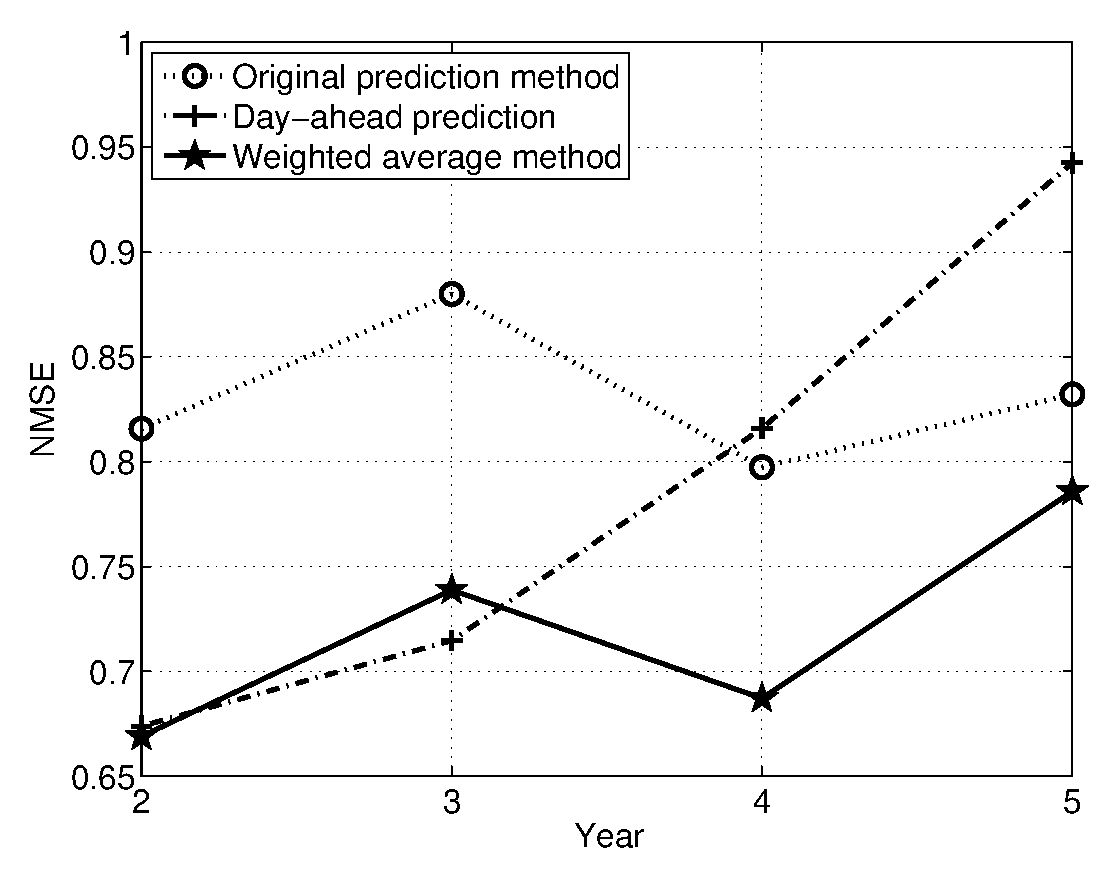
\includegraphics[width = 0.8\textwidth]{fig/err_r_compare.eps}
  \caption{Prediction Performance (Electricity Price).}
\end{figure}

The prediction error is computed by normalize mean square error (NMSE) for each year, i.e.,
\begin{equation*}
    \text{NMSE} = \frac{\frac{1}{365}\sum_{d = 1}^{365}\frac{1}{24}\sum_{h=1}^{24}(\hat x_d(h)-x_d(h))^2}{\frac{1}{365}\sum_{d = 1}^{365}\frac{1}{24}\sum_{h=1}^{24}(\bar x(h)-x_d(h))^2} = \frac{\sum_{d = 1}^{365}\sum_{h=1}^{24}(\hat x_d(h)-x_d(h))^2}{\sum_{d = 1}^{365}\sum_{h=1}^{24}(\bar x(h)-x_d(h))^2}.
\end{equation*}
The NMSE is fair to compare the estimator for different data since variance are much different in different data or years. To see the long-term performance, we generate also 5 years of synthesized data obtained with random linear combinations
of the data from 2010 to 2014, i.e.,
\begin{equation}
    \bfx_{365\times(y-1)+d} = \sum_{i=1}^5 z_i\bfx_{365\times(i-1)+d}
\end{equation}
where $d=1,\ldots,365$, $y=6,\ldots,10$, and $z_i$ are random generated from uniform distribution in $[0,1]$ and normalize such that $z_1+\ldots+z_5=1$. The detail method is shown in algorithm~\ref{algo: synthesized data}.

\begin{algorithm}[!t]
    \label{algo: synthesized data}
    \caption{Synthesized Data}
    \For{\bf{each} $y\in \{6,7,8,9,10\}$}{
        $z_i = \calU(0,1), i = 1,\ldots,5$\\
        $z_i = z_i/\sum_{i'=1}^5{z_i'}, i = 1,\ldots,5$\\
        \For{\bf{each} $d\in \{1,2,\ldots,365\}$}{
            $\bfx_{365\times(y-1)+d} = \sum_{i=1}^5 z_i\bfx_{365\times(i-1)+d}$
        }
    }
\end{algorithm}

In the end of this chapter, we summarize the proposed algorithm in Algorithm~\ref{algo: EMS-LSPI}. In step 1, we initial the policy for different year. The first year is the training data which is applied equal cost policy and 6 random policy (equal cost policy and random policy will introduce in Chapter~\ref{cha: Simulation}). The year $e$ is used to enhance the training data in first year since we utilize the weight obtained by first year to testing the training data. After the second year, we apply LSPI with perfect prediction in our training data. In step 2, we initial the previous state for different year since the first states are not the same in different year (the first state in the second year is obtained by equal cost policy and the first state in the third year is obtained by LSPI). In step 3, we generate the samples in each year and testing except first year. This step is a simple loop to generate the triple $(\bfs_d,\bfalpha_{d+1},\bfs_{d+1})$ by using different policy. In step 5, we adopt the LSPI algorithm to obtain the weight of basis.

\newgeometry{top=4em,left=3em,right=2.5em}
\begin{algorithm}[t]
    \caption{EMS-LSPI}
    \label{algo: EMS-LSPI}

    \For{{\bf each} $y\in\{1,e,2,3,4,5\}$}{

        \tcc{Step 1: Initial policy name}
        \uIf{$y=1$}{
            $\Pi\leftarrow$ \{equal cost policy, 6 random policy\}
        }
        \uElseIf{$y=e$}{
            $\Pi\leftarrow$ \{LSPI, 6 random policy\}
        }
        \Else{
            $\Pi\leftarrow$ \{LSPI, LSPI with perfect prediction, equal cost policy, 6 random policy\}
        }

        \tcc{Step 2: Initial previous state}
        \uIf{$y=1$ {\bf or} $y=e$}{
            $\bfs_\text{prev}\leftarrow (\bfr_1,\bfx_1,\bfp^\tDA_2,\bfp^\tRT_1,\bfb_1)$ where $b_1(h) = C$ for all $h$.
        }
        \uElseIf{$y=2$}{
            $\bfs_\text{prev}\leftarrow (\bfr_d,\bfx_d,\bfp^\tDA_{d+1},\bfp^\tRT_d,\bfb^\pi_d)$ where $d = 365\times(y-1)+1$ and $\pi$ is equal cost policy.
        }
        \Else{
            $\bfs_\text{prev}\leftarrow (\bfr_d,\bfx_d,\bfp^\tDA_{d+1},\bfp^\tRT_d,\bfb^\pi_d)$ where $d = 365\times(y-1)+1$ and $\pi$ is LSPI.
        }

        \tcc{Step 3: Generate samples (each year) and testing (except first year)}
        \For{{\bf each} $d\in \{365\times(y-1)+1,\ldots,365\times(y-1)+365\}$}{

            \tcc{Set state for day $d$ (current state)}
            $\bfs_d \leftarrow  \bfs_\text{prev}$\\

            \tcc{Set action for next day}
            \For{{\bf each} $\pi\in\Pi$}{
                \uIf{$\pi=$ LSPI}{
                    $\bfalpha^\pi_{d+1} \leftarrow \arg\max_{\bfalpha'}\widehat{Q}(T_r(\bfs_d, \bfalpha'), T_x(\bfs_d, \bfalpha'), \bfp^\tDA_{d+1}, T_{p^\tRT}(\bfs_d, \bfalpha'), T_b(\bfs_d, \bfalpha'), \bfalpha_{d+1}, \bfs_d; \bfw^*)$
                }
                \uElseIf{$\pi=$ LSPI with perfect prediction}{
                    $\bfalpha^\pi_{d+1} \leftarrow \arg\max_{\bfalpha'}\widehat{Q}(T_r(\bfs_d, \bfalpha'), T_x(\bfs_d, \bfalpha'), \bfp^\tDA_{d+1}, T_{p^\tRT}(\bfs_d, \bfalpha'), T_b(\bfs_d, \bfalpha'), \bfalpha_{d+1}, \bfs_d; \bfw^*)$
                }
                \uElseIf{$\pi=$ equal cost policy}{
                    $\bfalpha^\pi_{d+1}(h) \leftarrow \frac{1/\hat{p}^\text{DA}_{d+1}(h)}{\sum_{h_2=1}^{24} 1/\hat{p}^\text{DA}_{d+1}(h_2)}\sum_{h_1=1}^{24}(\hat x_{d+1}(h_1)-\hat r_{d+1}(h_1))$
                }
                \ElseIf{$\pi=$ random policy}{
                    $\bfalpha^\pi_{d+1}(h) \leftarrow \calU(\mu^\text{LSPI}_{d+1}(h) - 1.5\sigma^\text{LSPI}_{d+1}(h), \mu^\text{LSPI}_{d+1}(h) + 1.5\sigma^\text{LSPI}_{d+1}(h))$ where $\pi'$ is equal cost policy if $y=1$, otherwise, $\pi'$ is the LSPI policy.
                }

                ${\bfs'}^\pi_{d+1} \leftarrow (\bfr_{d+1},\bfx_{d+1},\bfp^\text{DA}_{d+2},\bfp^\text{RT}_{d+1},\bfb^\pi_{d+1})$\tcc*[r]{Set state for next day (next state)}

                $r^\pi_{d+1} \leftarrow -\kappa_{d+1}$\tcc*[r]{Set reward for next day (for this transition)}
            }

            \tcc{Initial previous state}
            \eIf{$y=1$}{
                $\bfs_\text{prev} \leftarrow {\bfs'}^\pi_{d+1}$ where $\pi$ is equal cost policy.
            }{
                $\bfs_\text{prev} \leftarrow {\bfs'}^\pi_{d+1}$ where $\pi$ is LSPI.
            }
        }
        \tcc{Step 4: LSPI algorithm}
        \If{$y=5$}{
            break for loop \tcc*[r]{No need to training last year}
        }
        $\calD\leftarrow\{(\bfs_d,\bfalpha^\pi_{d+1},{\bfs'}^\pi_{d+1},r^\pi_{d+1})\}_{\pi\in\Pi, d\in \{1,2,\ldots,365\times(y-1)+365\}}$\\
        $\bfw^*\leftarrow \text{LSPI}(\calD, \bfphi, \gamma, \epsilon)$\\
    }
\end{algorithm}
\restoregeometry
\baselineskip 24pt
